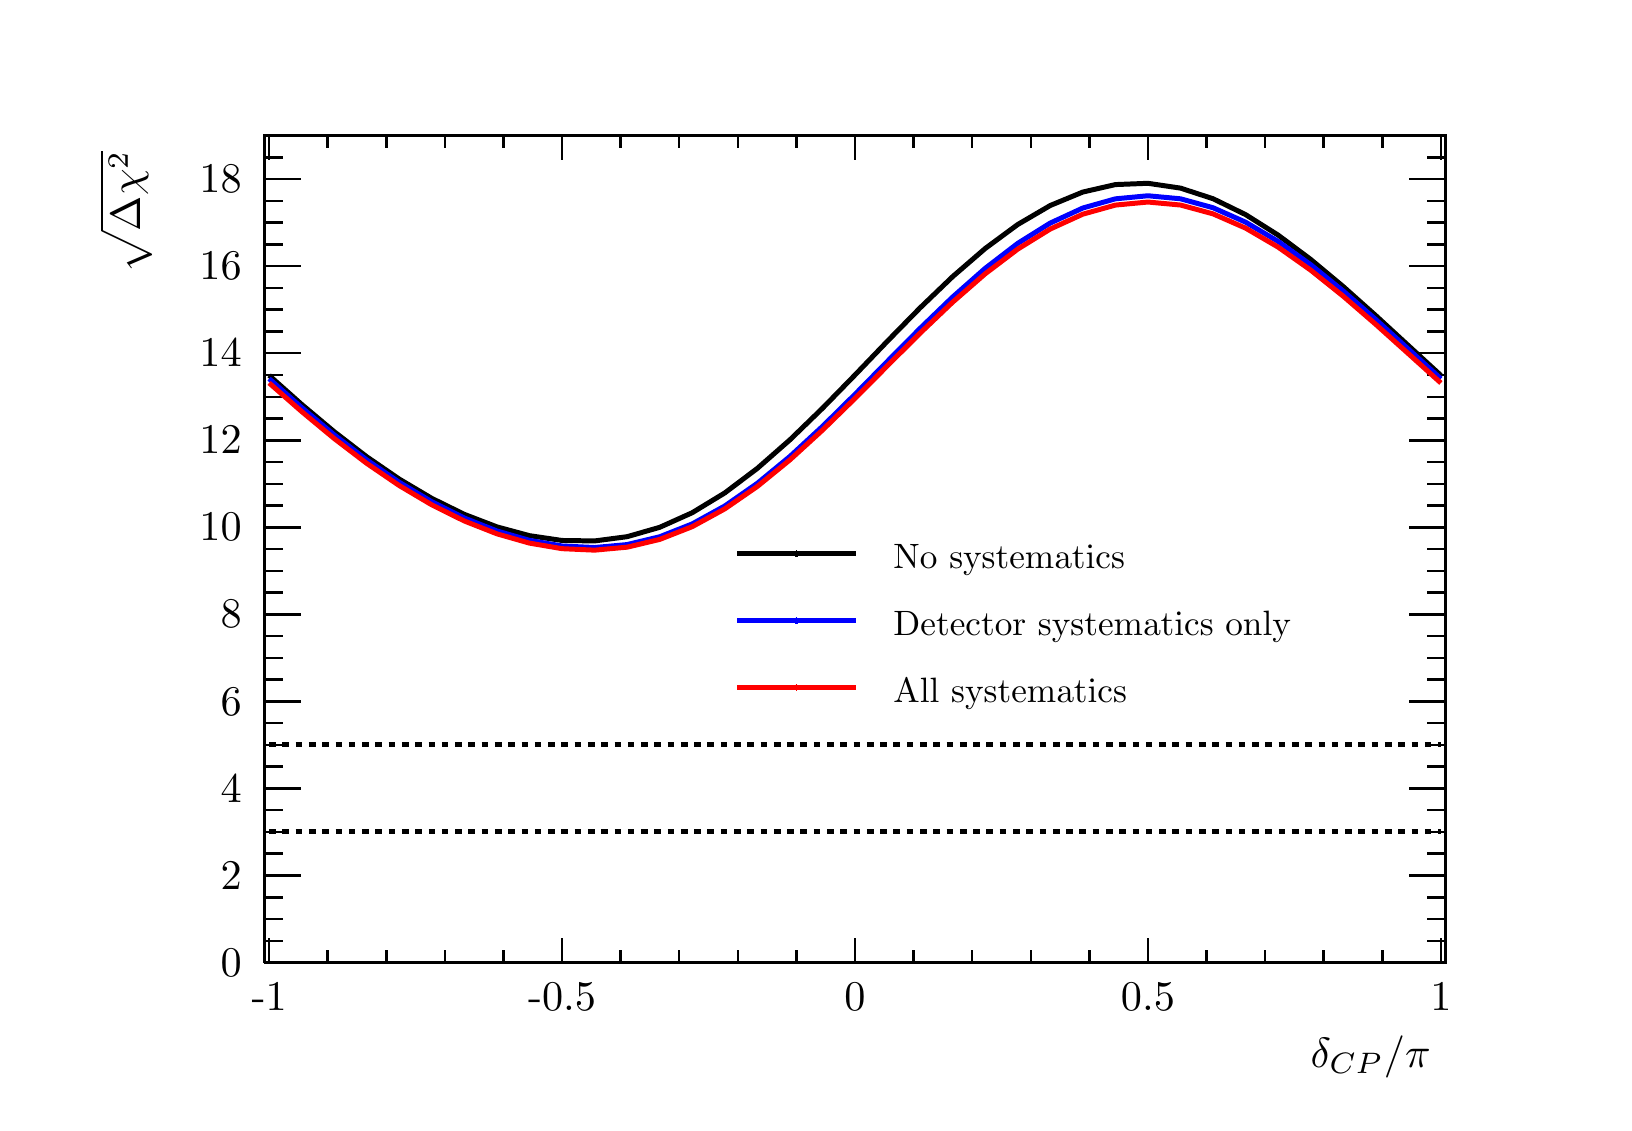
\begin{tikzpicture}
\pgfdeclareplotmark{cross} {
\pgfpathmoveto{\pgfpoint{-0.3\pgfplotmarksize}{\pgfplotmarksize}}
\pgfpathlineto{\pgfpoint{+0.3\pgfplotmarksize}{\pgfplotmarksize}}
\pgfpathlineto{\pgfpoint{+0.3\pgfplotmarksize}{0.3\pgfplotmarksize}}
\pgfpathlineto{\pgfpoint{+1\pgfplotmarksize}{0.3\pgfplotmarksize}}
\pgfpathlineto{\pgfpoint{+1\pgfplotmarksize}{-0.3\pgfplotmarksize}}
\pgfpathlineto{\pgfpoint{+0.3\pgfplotmarksize}{-0.3\pgfplotmarksize}}
\pgfpathlineto{\pgfpoint{+0.3\pgfplotmarksize}{-1.\pgfplotmarksize}}
\pgfpathlineto{\pgfpoint{-0.3\pgfplotmarksize}{-1.\pgfplotmarksize}}
\pgfpathlineto{\pgfpoint{-0.3\pgfplotmarksize}{-0.3\pgfplotmarksize}}
\pgfpathlineto{\pgfpoint{-1.\pgfplotmarksize}{-0.3\pgfplotmarksize}}
\pgfpathlineto{\pgfpoint{-1.\pgfplotmarksize}{0.3\pgfplotmarksize}}
\pgfpathlineto{\pgfpoint{-0.3\pgfplotmarksize}{0.3\pgfplotmarksize}}
\pgfpathclose
\pgfusepathqstroke
}
\pgfdeclareplotmark{cross*} {
\pgfpathmoveto{\pgfpoint{-0.3\pgfplotmarksize}{\pgfplotmarksize}}
\pgfpathlineto{\pgfpoint{+0.3\pgfplotmarksize}{\pgfplotmarksize}}
\pgfpathlineto{\pgfpoint{+0.3\pgfplotmarksize}{0.3\pgfplotmarksize}}
\pgfpathlineto{\pgfpoint{+1\pgfplotmarksize}{0.3\pgfplotmarksize}}
\pgfpathlineto{\pgfpoint{+1\pgfplotmarksize}{-0.3\pgfplotmarksize}}
\pgfpathlineto{\pgfpoint{+0.3\pgfplotmarksize}{-0.3\pgfplotmarksize}}
\pgfpathlineto{\pgfpoint{+0.3\pgfplotmarksize}{-1.\pgfplotmarksize}}
\pgfpathlineto{\pgfpoint{-0.3\pgfplotmarksize}{-1.\pgfplotmarksize}}
\pgfpathlineto{\pgfpoint{-0.3\pgfplotmarksize}{-0.3\pgfplotmarksize}}
\pgfpathlineto{\pgfpoint{-1.\pgfplotmarksize}{-0.3\pgfplotmarksize}}
\pgfpathlineto{\pgfpoint{-1.\pgfplotmarksize}{0.3\pgfplotmarksize}}
\pgfpathlineto{\pgfpoint{-0.3\pgfplotmarksize}{0.3\pgfplotmarksize}}
\pgfpathclose
\pgfusepathqfillstroke
}
\pgfdeclareplotmark{newstar} {
\pgfpathmoveto{\pgfqpoint{0pt}{\pgfplotmarksize}}
\pgfpathlineto{\pgfqpointpolar{44}{0.5\pgfplotmarksize}}
\pgfpathlineto{\pgfqpointpolar{18}{\pgfplotmarksize}}
\pgfpathlineto{\pgfqpointpolar{-20}{0.5\pgfplotmarksize}}
\pgfpathlineto{\pgfqpointpolar{-54}{\pgfplotmarksize}}
\pgfpathlineto{\pgfqpointpolar{-90}{0.5\pgfplotmarksize}}
\pgfpathlineto{\pgfqpointpolar{234}{\pgfplotmarksize}}
\pgfpathlineto{\pgfqpointpolar{198}{0.5\pgfplotmarksize}}
\pgfpathlineto{\pgfqpointpolar{162}{\pgfplotmarksize}}
\pgfpathlineto{\pgfqpointpolar{134}{0.5\pgfplotmarksize}}
\pgfpathclose
\pgfusepathqstroke
}
\pgfdeclareplotmark{newstar*} {
\pgfpathmoveto{\pgfqpoint{0pt}{\pgfplotmarksize}}
\pgfpathlineto{\pgfqpointpolar{44}{0.5\pgfplotmarksize}}
\pgfpathlineto{\pgfqpointpolar{18}{\pgfplotmarksize}}
\pgfpathlineto{\pgfqpointpolar{-20}{0.5\pgfplotmarksize}}
\pgfpathlineto{\pgfqpointpolar{-54}{\pgfplotmarksize}}
\pgfpathlineto{\pgfqpointpolar{-90}{0.5\pgfplotmarksize}}
\pgfpathlineto{\pgfqpointpolar{234}{\pgfplotmarksize}}
\pgfpathlineto{\pgfqpointpolar{198}{0.5\pgfplotmarksize}}
\pgfpathlineto{\pgfqpointpolar{162}{\pgfplotmarksize}}
\pgfpathlineto{\pgfqpointpolar{134}{0.5\pgfplotmarksize}}
\pgfpathclose
\pgfusepathqfillstroke
}
\definecolor{c}{rgb}{1,1,1};
\draw [color=c, fill=c] (0,0) rectangle (20,13.639);
\draw [color=c, fill=c] (3,1.77307) rectangle (18,12.2751);
\definecolor{c}{rgb}{0,0,0};
\draw [c,line width=0.9] (3,1.77307) -- (3,12.2751) -- (18,12.2751) -- (18,1.77307) -- (3,1.77307);
\definecolor{c}{rgb}{1,1,1};
\draw [color=c, fill=c] (3,1.77307) rectangle (18,12.2751);
\definecolor{c}{rgb}{0,0,0};
\draw [c,line width=0.9] (3,1.77307) -- (3,12.2751) -- (18,12.2751) -- (18,1.77307) -- (3,1.77307);
\draw [c,line width=0.9] (3,1.77307) -- (18,1.77307);
\draw [c,line width=0.9] (3.05952,2.07994) -- (3.05952,1.77307);
\draw [c,line width=0.9] (3.80357,1.9265) -- (3.80357,1.77307);
\draw [c,line width=0.9] (4.54762,1.9265) -- (4.54762,1.77307);
\draw [c,line width=0.9] (5.29167,1.9265) -- (5.29167,1.77307);
\draw [c,line width=0.9] (6.03571,1.9265) -- (6.03571,1.77307);
\draw [c,line width=0.9] (6.77976,2.07994) -- (6.77976,1.77307);
\draw [c,line width=0.9] (7.52381,1.9265) -- (7.52381,1.77307);
\draw [c,line width=0.9] (8.26786,1.9265) -- (8.26786,1.77307);
\draw [c,line width=0.9] (9.0119,1.9265) -- (9.0119,1.77307);
\draw [c,line width=0.9] (9.75595,1.9265) -- (9.75595,1.77307);
\draw [c,line width=0.9] (10.5,2.07994) -- (10.5,1.77307);
\draw [c,line width=0.9] (11.244,1.9265) -- (11.244,1.77307);
\draw [c,line width=0.9] (11.9881,1.9265) -- (11.9881,1.77307);
\draw [c,line width=0.9] (12.7321,1.9265) -- (12.7321,1.77307);
\draw [c,line width=0.9] (13.4762,1.9265) -- (13.4762,1.77307);
\draw [c,line width=0.9] (14.2202,2.07994) -- (14.2202,1.77307);
\draw [c,line width=0.9] (14.9643,1.9265) -- (14.9643,1.77307);
\draw [c,line width=0.9] (15.7083,1.9265) -- (15.7083,1.77307);
\draw [c,line width=0.9] (16.4524,1.9265) -- (16.4524,1.77307);
\draw [c,line width=0.9] (17.1964,1.9265) -- (17.1964,1.77307);
\draw [c,line width=0.9] (17.9405,2.07994) -- (17.9405,1.77307);
\draw [c,line width=0.9] (3.05952,2.07994) -- (3.05952,1.77307);
\draw [c,line width=0.9] (17.9405,2.07994) -- (17.9405,1.77307);
\draw [anchor=base] (3.05952,1.15931) node[scale=1.52731, color=c, rotate=0]{-1};
\draw [anchor=base] (6.77976,1.15931) node[scale=1.52731, color=c, rotate=0]{-0.5};
\draw [anchor=base] (10.5,1.15931) node[scale=1.52731, color=c, rotate=0]{0};
\draw [anchor=base] (14.2202,1.15931) node[scale=1.52731, color=c, rotate=0]{0.5};
\draw [anchor=base] (17.9405,1.15931) node[scale=1.52731, color=c, rotate=0]{1};
\draw [anchor= east] (18,0.572837) node[scale=1.52731, color=c, rotate=0]{$\delta_{CP} / \pi$};
\draw [c,line width=0.9] (3,12.2751) -- (18,12.2751);
\draw [c,line width=0.9] (3.05952,11.9682) -- (3.05952,12.2751);
\draw [c,line width=0.9] (3.80357,12.1216) -- (3.80357,12.2751);
\draw [c,line width=0.9] (4.54762,12.1216) -- (4.54762,12.2751);
\draw [c,line width=0.9] (5.29167,12.1216) -- (5.29167,12.2751);
\draw [c,line width=0.9] (6.03571,12.1216) -- (6.03571,12.2751);
\draw [c,line width=0.9] (6.77976,11.9682) -- (6.77976,12.2751);
\draw [c,line width=0.9] (7.52381,12.1216) -- (7.52381,12.2751);
\draw [c,line width=0.9] (8.26786,12.1216) -- (8.26786,12.2751);
\draw [c,line width=0.9] (9.0119,12.1216) -- (9.0119,12.2751);
\draw [c,line width=0.9] (9.75595,12.1216) -- (9.75595,12.2751);
\draw [c,line width=0.9] (10.5,11.9682) -- (10.5,12.2751);
\draw [c,line width=0.9] (11.244,12.1216) -- (11.244,12.2751);
\draw [c,line width=0.9] (11.9881,12.1216) -- (11.9881,12.2751);
\draw [c,line width=0.9] (12.7321,12.1216) -- (12.7321,12.2751);
\draw [c,line width=0.9] (13.4762,12.1216) -- (13.4762,12.2751);
\draw [c,line width=0.9] (14.2202,11.9682) -- (14.2202,12.2751);
\draw [c,line width=0.9] (14.9643,12.1216) -- (14.9643,12.2751);
\draw [c,line width=0.9] (15.7083,12.1216) -- (15.7083,12.2751);
\draw [c,line width=0.9] (16.4524,12.1216) -- (16.4524,12.2751);
\draw [c,line width=0.9] (17.1964,12.1216) -- (17.1964,12.2751);
\draw [c,line width=0.9] (17.9405,11.9682) -- (17.9405,12.2751);
\draw [c,line width=0.9] (3.05952,11.9682) -- (3.05952,12.2751);
\draw [c,line width=0.9] (17.9405,11.9682) -- (17.9405,12.2751);
\draw [c,line width=0.9] (3,1.77307) -- (3,12.2751);
\draw [c,line width=0.9] (3.462,1.77307) -- (3,1.77307);
\draw [c,line width=0.9] (3.231,2.04943) -- (3,2.04943);
\draw [c,line width=0.9] (3.231,2.3258) -- (3,2.3258);
\draw [c,line width=0.9] (3.231,2.60217) -- (3,2.60217);
\draw [c,line width=0.9] (3.462,2.87854) -- (3,2.87854);
\draw [c,line width=0.9] (3.231,3.15491) -- (3,3.15491);
\draw [c,line width=0.9] (3.231,3.43128) -- (3,3.43128);
\draw [c,line width=0.9] (3.231,3.70765) -- (3,3.70765);
\draw [c,line width=0.9] (3.462,3.98401) -- (3,3.98401);
\draw [c,line width=0.9] (3.231,4.26038) -- (3,4.26038);
\draw [c,line width=0.9] (3.231,4.53675) -- (3,4.53675);
\draw [c,line width=0.9] (3.231,4.81312) -- (3,4.81312);
\draw [c,line width=0.9] (3.462,5.08949) -- (3,5.08949);
\draw [c,line width=0.9] (3.231,5.36586) -- (3,5.36586);
\draw [c,line width=0.9] (3.231,5.64223) -- (3,5.64223);
\draw [c,line width=0.9] (3.231,5.91859) -- (3,5.91859);
\draw [c,line width=0.9] (3.462,6.19496) -- (3,6.19496);
\draw [c,line width=0.9] (3.231,6.47133) -- (3,6.47133);
\draw [c,line width=0.9] (3.231,6.7477) -- (3,6.7477);
\draw [c,line width=0.9] (3.231,7.02407) -- (3,7.02407);
\draw [c,line width=0.9] (3.462,7.30044) -- (3,7.30044);
\draw [c,line width=0.9] (3.231,7.57681) -- (3,7.57681);
\draw [c,line width=0.9] (3.231,7.85317) -- (3,7.85317);
\draw [c,line width=0.9] (3.231,8.12954) -- (3,8.12954);
\draw [c,line width=0.9] (3.462,8.40591) -- (3,8.40591);
\draw [c,line width=0.9] (3.231,8.68228) -- (3,8.68228);
\draw [c,line width=0.9] (3.231,8.95865) -- (3,8.95865);
\draw [c,line width=0.9] (3.231,9.23502) -- (3,9.23502);
\draw [c,line width=0.9] (3.462,9.51139) -- (3,9.51139);
\draw [c,line width=0.9] (3.231,9.78775) -- (3,9.78775);
\draw [c,line width=0.9] (3.231,10.0641) -- (3,10.0641);
\draw [c,line width=0.9] (3.231,10.3405) -- (3,10.3405);
\draw [c,line width=0.9] (3.462,10.6169) -- (3,10.6169);
\draw [c,line width=0.9] (3.231,10.8932) -- (3,10.8932);
\draw [c,line width=0.9] (3.231,11.1696) -- (3,11.1696);
\draw [c,line width=0.9] (3.231,11.446) -- (3,11.446);
\draw [c,line width=0.9] (3.462,11.7223) -- (3,11.7223);
\draw [c,line width=0.9] (3.462,11.7223) -- (3,11.7223);
\draw [c,line width=0.9] (3.231,11.9987) -- (3,11.9987);
\draw [c,line width=0.9] (3.231,12.2751) -- (3,12.2751);
\draw [anchor= east] (2.9,1.77307) node[scale=1.52731, color=c, rotate=0]{0};
\draw [anchor= east] (2.9,2.87854) node[scale=1.52731, color=c, rotate=0]{2};
\draw [anchor= east] (2.9,3.98401) node[scale=1.52731, color=c, rotate=0]{4};
\draw [anchor= east] (2.9,5.08949) node[scale=1.52731, color=c, rotate=0]{6};
\draw [anchor= east] (2.9,6.19496) node[scale=1.52731, color=c, rotate=0]{8};
\draw [anchor= east] (2.9,7.30044) node[scale=1.52731, color=c, rotate=0]{10};
\draw [anchor= east] (2.9,8.40591) node[scale=1.52731, color=c, rotate=0]{12};
\draw [anchor= east] (2.9,9.51139) node[scale=1.52731, color=c, rotate=0]{14};
\draw [anchor= east] (2.9,10.6169) node[scale=1.52731, color=c, rotate=0]{16};
\draw [anchor= east] (2.9,11.7223) node[scale=1.52731, color=c, rotate=0]{18};
\draw [anchor= east] (1.24,12.2751) node[scale=1.52731, color=c, rotate=90]{$\sqrt{ \Delta \chi^{2} }$};
\draw [c,line width=0.9] (18,1.77307) -- (18,12.2751);
\draw [c,line width=0.9] (17.538,1.77307) -- (18,1.77307);
\draw [c,line width=0.9] (17.769,2.04943) -- (18,2.04943);
\draw [c,line width=0.9] (17.769,2.3258) -- (18,2.3258);
\draw [c,line width=0.9] (17.769,2.60217) -- (18,2.60217);
\draw [c,line width=0.9] (17.538,2.87854) -- (18,2.87854);
\draw [c,line width=0.9] (17.769,3.15491) -- (18,3.15491);
\draw [c,line width=0.9] (17.769,3.43128) -- (18,3.43128);
\draw [c,line width=0.9] (17.769,3.70765) -- (18,3.70765);
\draw [c,line width=0.9] (17.538,3.98401) -- (18,3.98401);
\draw [c,line width=0.9] (17.769,4.26038) -- (18,4.26038);
\draw [c,line width=0.9] (17.769,4.53675) -- (18,4.53675);
\draw [c,line width=0.9] (17.769,4.81312) -- (18,4.81312);
\draw [c,line width=0.9] (17.538,5.08949) -- (18,5.08949);
\draw [c,line width=0.9] (17.769,5.36586) -- (18,5.36586);
\draw [c,line width=0.9] (17.769,5.64223) -- (18,5.64223);
\draw [c,line width=0.9] (17.769,5.91859) -- (18,5.91859);
\draw [c,line width=0.9] (17.538,6.19496) -- (18,6.19496);
\draw [c,line width=0.9] (17.769,6.47133) -- (18,6.47133);
\draw [c,line width=0.9] (17.769,6.7477) -- (18,6.7477);
\draw [c,line width=0.9] (17.769,7.02407) -- (18,7.02407);
\draw [c,line width=0.9] (17.538,7.30044) -- (18,7.30044);
\draw [c,line width=0.9] (17.769,7.57681) -- (18,7.57681);
\draw [c,line width=0.9] (17.769,7.85317) -- (18,7.85317);
\draw [c,line width=0.9] (17.769,8.12954) -- (18,8.12954);
\draw [c,line width=0.9] (17.538,8.40591) -- (18,8.40591);
\draw [c,line width=0.9] (17.769,8.68228) -- (18,8.68228);
\draw [c,line width=0.9] (17.769,8.95865) -- (18,8.95865);
\draw [c,line width=0.9] (17.769,9.23502) -- (18,9.23502);
\draw [c,line width=0.9] (17.538,9.51139) -- (18,9.51139);
\draw [c,line width=0.9] (17.769,9.78775) -- (18,9.78775);
\draw [c,line width=0.9] (17.769,10.0641) -- (18,10.0641);
\draw [c,line width=0.9] (17.769,10.3405) -- (18,10.3405);
\draw [c,line width=0.9] (17.538,10.6169) -- (18,10.6169);
\draw [c,line width=0.9] (17.769,10.8932) -- (18,10.8932);
\draw [c,line width=0.9] (17.769,11.1696) -- (18,11.1696);
\draw [c,line width=0.9] (17.769,11.446) -- (18,11.446);
\draw [c,line width=0.9] (17.538,11.7223) -- (18,11.7223);
\draw [c,line width=0.9] (17.538,11.7223) -- (18,11.7223);
\draw [c,line width=0.9] (17.769,11.9987) -- (18,11.9987);
\draw [c,line width=0.9] (17.769,12.2751) -- (18,12.2751);
\draw [c,line width=1.8] (3.05952,9.22955) -- (3.47288,8.86155) -- (3.88624,8.5146) -- (4.2996,8.19636) -- (4.71296,7.91266) -- (5.12632,7.66774) -- (5.53968,7.46466) -- (5.95304,7.30597) -- (6.3664,7.19439) -- (6.77976,7.13339) -- (7.19312,7.12746)
 -- (7.60648,7.18165) -- (8.01984,7.30045) -- (8.4332,7.48617) -- (8.84656,7.73754) -- (9.25992,8.04911) -- (9.67328,8.41145) -- (10.0866,8.81184) -- (10.5,9.23541) -- (10.9134,9.66611) -- (11.3267,10.0877) -- (11.7401,10.4843) -- (12.1534,10.8414)
 -- (12.5668,11.1461) -- (12.9802,11.3878) -- (13.3935,11.5585) -- (13.8069,11.6531) -- (14.2202,11.6694) -- (14.6336,11.6083) -- (15.047,11.4736) -- (15.4603,11.2718) -- (15.8737,11.0114) -- (16.287,10.7029) -- (16.7004,10.3581) -- (17.1138,9.98932)
 -- (17.5271,9.60913) -- (17.9405,9.22955);
\definecolor{c}{rgb}{0,0,1};
\draw [c,line width=1.8] (3.05952,9.18742) -- (3.47288,8.82099) -- (3.88624,8.47464) -- (4.2996,8.15621) -- (4.71296,7.87152) -- (5.12632,7.62453) -- (5.53968,7.41795) -- (5.95304,7.25387) -- (6.3664,7.1346) -- (6.77976,7.06325) -- (7.19312,7.04395)
 -- (7.60648,7.08154) -- (8.01984,7.18056) -- (8.4332,7.34397) -- (8.84656,7.57167) -- (9.25992,7.85973) -- (9.67328,8.20018) -- (10.0866,8.58148) -- (10.5,8.98951) -- (10.9134,9.40989) -- (11.3267,9.82699) -- (11.7401,10.2251) -- (12.1534,10.5895)
 -- (12.5668,10.9066) -- (12.9802,11.1649) -- (13.3935,11.3556) -- (13.8069,11.4721) -- (14.2202,11.5112) -- (14.6336,11.4726) -- (15.047,11.3591) -- (15.4603,11.176) -- (15.8737,10.9316) -- (16.287,10.636) -- (16.7004,10.3011) -- (17.1138,9.9395) --
 (17.5271,9.5641) -- (17.9405,9.18742);
\definecolor{c}{rgb}{1,0,0};
\draw [c,line width=1.8] (3.05952,9.13367) -- (3.47288,8.77085) -- (3.88624,8.42775) -- (4.2996,8.11218) -- (4.71296,7.82997) -- (5.12632,7.58509) -- (5.53968,7.38027) -- (5.95304,7.21765) -- (6.3664,7.09959) -- (6.77976,7.02918) -- (7.19312,7.01049)
 -- (7.60648,7.04822) -- (8.01984,7.14678) -- (8.4332,7.30899) -- (8.84656,7.53471) -- (9.25992,7.81999) -- (9.67328,8.15697) -- (10.0866,8.53433) -- (10.5,8.93807) -- (10.9134,9.35378) -- (11.3267,9.76616) -- (11.7401,10.1598) -- (12.1534,10.52) --
 (12.5668,10.8335) -- (12.9802,11.089) -- (13.3935,11.2775) -- (13.8069,11.3928) -- (14.2202,11.4315) -- (14.6336,11.3935) -- (15.047,11.2813) -- (15.4603,11.1004) -- (15.8737,10.8588) -- (16.287,10.5667) -- (16.7004,10.2355) -- (17.1138,9.87787) --
 (17.5271,9.50646) -- (17.9405,9.13367);
\definecolor{c}{rgb}{0,0,0};
\draw [c,dash pattern=on 2.40pt off 2.40pt ,line width=1.8] (3.05952,3.43128) -- (17.9405,3.43128);
\draw [c,dash pattern=on 2.40pt off 2.40pt ,line width=1.8] (3.05952,4.53675) -- (17.9405,4.53675);
\definecolor{c}{rgb}{1,1,1};
\draw [color=c, fill=c] (8.68195,4.84241) rectangle (17.2779,7.39255);
\definecolor{c}{rgb}{0,0,0};
\draw [anchor=base west] (10.8309,6.77627) node[scale=1.27276, color=c, rotate=0]{No systematics};
\definecolor{c}{rgb}{1,1,1};
\draw [c, fill=c] (9.0043,6.67001) -- (10.5086,6.67001) -- (10.5086,7.26504) -- (9.0043,7.26504);
\definecolor{c}{rgb}{0,0,0};
\draw [c,line width=1.8] (9.0043,6.96753) -- (10.5086,6.96753);
\foreach \P in {(9.75645,6.96753)}{\draw[mark options={color=c,fill=c},mark size=2.402402pt, line width=0.000000pt, mark=*,mark size=1pt] plot coordinates {\P};}
\draw [anchor=base west] (10.8309,5.92622) node[scale=1.27276, color=c, rotate=0]{Detector systematics only};
\definecolor{c}{rgb}{1,1,1};
\draw [c, fill=c] (9.0043,5.81996) -- (10.5086,5.81996) -- (10.5086,6.415) -- (9.0043,6.415);
\definecolor{c}{rgb}{0,0,1};
\draw [c,line width=1.8] (9.0043,6.11748) -- (10.5086,6.11748);
\foreach \P in {(9.75645,6.11748)}{\draw[mark options={color=c,fill=c},mark size=2.402402pt, line width=0.000000pt, mark=*,mark size=1pt] plot coordinates {\P};}
\definecolor{c}{rgb}{0,0,0};
\draw [anchor=base west] (10.8309,5.07617) node[scale=1.27276, color=c, rotate=0]{All systematics};
\definecolor{c}{rgb}{1,1,1};
\draw [c, fill=c] (9.0043,4.96991) -- (10.5086,4.96991) -- (10.5086,5.56495) -- (9.0043,5.56495);
\definecolor{c}{rgb}{1,0,0};
\draw [c,line width=1.8] (9.0043,5.26743) -- (10.5086,5.26743);
\foreach \P in {(9.75645,5.26743)}{\draw[mark options={color=c,fill=c},mark size=2.402402pt, line width=0.000000pt, mark=*,mark size=1pt] plot coordinates {\P};}
\end{tikzpicture}
